%%%%%%%%%%%%%%%%%%%%%%%%%%%%%%%%%%%%%%%%%
% Masters/Doctoral Thesis
% LaTeX Template
% Version 2.5 (27/8/17)
%
% This template was downloaded from:
% http://www.LaTeXTemplates.com
%
% Version 2.x major modifications by:
% Vel (vel@latextemplates.com)
%
% This template is based on a template by:
% Steve Gunn (http://users.ecs.soton.ac.uk/srg/softwaretools/document/templates/)
% Sunil Patel (http://www.sunilpatel.co.uk/thesis-template/)
%
% Template license:
% CC BY-NC-SA 3.0 (http://creativecommons.org/licenses/by-nc-sa/3.0/)
%
%%%%%%%%%%%%%%%%%%%%%%%%%%%%%%%%%%%%%%%%%

%----------------------------------------------------------------------------------------
%	PACKAGES AND OTHER DOCUMENT CONFIGURATIONS
%----------------------------------------------------------------------------------------

\documentclass[
12pt, % The default document font size, options: 10pt, 11pt, 12pt
%oneside, % Two side (alternating margins) for binding by default, uncomment to switch to one side
english, % ngerman for German
singlespacing, % Single line spacing, alternatives: onehalfspacing or doublespacing
%draft, % Uncomment to enable draft mode (no pictures, no links, overfull hboxes indicated)
%nolistspacing, % If the document is onehalfspacing or doublespacing, uncomment this to set spacing in lists to single
%liststotoc, % Uncomment to add the list of figures/tables/etc to the table of contents
%toctotoc, % Uncomment to add the main table of contents to the table of contents
%parskip, % Uncomment to add space between paragraphs
%nohyperref, % Uncomment to not load the hyperref package
headsepline, % Uncomment to get a line under the header
%chapterinoneline, % Uncomment to place the chapter title next to the number on one line
%consistentlayout, % Uncomment to change the layout of the declaration, abstract and acknowledgements pages to match the default layout
]{MastersDoctoralThesis} % The class file specifying the document structure

\usepackage[utf8]{inputenc} % Required for inputting international characters
\usepackage[T1]{fontenc} % Output font encoding for international characters
\usepackage{fontspec}
\usepackage{lipsum,etoolbox}
\usepackage{makeidx}
\usepackage{amssymb}

\setmainfont{Times New Roman}
%\usepackage{mathpazo} % Use the Palatino font by default

%\usepackage[backend=bibtex,style=au{biblatex} % Use the bibtex backend with the authoryear citation style (which resembles APA)

\usepackage[backend=biber, style=ieee]{biblatex}
\addbibresource{Thesis.bib} % The filename of the bibliography

%\bibliographystyle{plain}
%\bibliography{Thesis}


\usepackage[autostyle=true]{csquotes} % Required to generate language-dependent quotes in the bibliography

%----------------------------------------------------------
%Patched Commands
%---------------------------------------------------------
%Add abstract to toc
\patchcmd{\abstract}{\titlepage}{\titlepage
\addcontentsline{toc}{chapter}{Abstract}}{}{}

%----------------------------------------------------------------------------------------
%	MARGIN SETTINGS
%----------------------------------------------------------------------------------------

\geometry{
	paper=a4paper, % Change to letterpaper for US letter
	inner=2.5cm, % Inner margin
	outer=3.8cm, % Outer margin
	bindingoffset=.5cm, % Binding offset
	top=1.5cm, % Top margin
	bottom=1.5cm, % Bottom margin
	%showframe, % Uncomment to show how the type block is set on the page
}

%----------------------------------------------------------------------------------------
%	THESIS INFORMATION
%----------------------------------------------------------------------------------------

\thesistitle{A comparison of metalearning strategies} % Your thesis title, this is used in the title and abstract, print it elsewhere with \ttitle
\supervisor{Dr. Thomas Smolinski \textsc{Smith}} % Your supervisor's name, this is used in the title page, print it elsewhere with \supname
\examiner{} % Your examiner's name, this is not currently used anywhere in the template, print it elsewhere with \examname
\degree{Masters in Science} % Your degree name, this is used in the title page and abstract, print it elsewhere with \degreename
\author{John \textsc{Liddell}} % Your name, this is used in the title page and abstract, print it elsewhere with \authorname
\addresses{} % Your address, this is not currently used anywhere in the template, print it elsewhere with \addressname

\subject{Computer Science} % Your subject area, this is not currently used anywhere in the template, print it elsewhere with \subjectname
\keywords{} % Keywords for your thesis, this is not currently used anywhere in the template, print it elsewhere with \keywordnames
\university{\href{http://www.desu.edu}{Delaware State University}} % Your university's name and URL, this is used in the title page and abstract, print it elsewhere with \univname
\department{\href{http://department.university}{Department of computer science}} % Your department's name and URL, this is used in the title page and abstract, print it elsewhere with \deptname
\group{\href{http://researchgroup.university.com}{CIBIL}} % Your research group's name and URL, this is used in the title page, print it elsewhere with \groupname
\faculty{\href{http://faculty.university.com}{Faculty Name}} % Your faculty's name and URL, this is used in the title page and abstract, print it elsewhere with \facname

\AtBeginDocument{
\hypersetup{pdftitle=\ttitle} % Set the PDF's title to your title
\hypersetup{pdfauthor=\authorname} % Set the PDF's author to your name
\hypersetup{pdfkeywords=\keywordnames} % Set the PDF's keywords to your keywords
}

\begin{document}

\frontmatter % Use roman page numbering style (i, ii, iii, iv...) for the pre-content pages

\pagestyle{plain} % Default to the plain heading style until the thesis style is called for the body content

%----------------------------------------------------------------------------------------
%	TITLE PAGE
%----------------------------------------------------------------------------------------

\begin{titlepage}
\begin{center}

\vspace*{.06\textheight}
{\scshape\LARGE \univname\par}\vspace{1.5cm} % University name
\textsc{\Large Masters Thesis}\\[0.5cm] % Thesis type

\HRule \\[0.4cm] % Horizontal line
{\huge \bfseries \ttitle\par}\vspace{0.4cm} % Thesis title
\HRule \\[1.5cm] % Horizontal line

\begin{minipage}[t]{0.4\textwidth}
\begin{flushleft} \large
\emph{Author:}\\
\end{flushleft}
\end{minipage}
\begin{minipage}[t]{0.4\textwidth}
\begin{flushright} \large
\emph{Supervisor:} \\
\end{flushright}
\end{minipage}\\[3cm]

\vfill

\large \textit{A thesis submitted in fulfillment of the requirements\\ for the degree of \degreename}\\[0.3cm] % University requirement text
\textit{in the}\\[0.4cm]
\groupname\\\deptname\\[2cm] % Research group name and department name

\vfill

{\large \today}\\[4cm] % Date
%\includegraphics{Logo} % University/department logo - uncomment to place it

\vfill
\end{center}
\end{titlepage}

%----------------------------------------------------------------------------------------
%	DECLARATION PAGE
%----------------------------------------------------------------------------------------

\begin{declaration}
\addchaptertocentry{\authorshipname} % Add the declaration to the table of contents
\noindent I, \authorname, declare that this thesis titled, \enquote{\ttitle} and the work presented in it are my own. I confirm that:

\begin{itemize}
\item This work was done wholly or mainly while in candidature for a research degree at this University.
\item Where any part of this thesis has previously been submitted for a degree or any other qualification at this University or any other institution, this has been clearly stated.
\item Where I have consulted the published work of others, this is always clearly attributed.
\item Where I have quoted from the work of others, the source is always given. With the exception of such quotations, this thesis is entirely my own work.
\item I have acknowledged all main sources of help.
\item Where the thesis is based on work done by myself jointly with others, I have made clear exactly what was done by others and what I have contributed myself.\\
\end{itemize}

\noindent Signed:\\
\rule[0.5em]{25em}{0.5pt} % This prints a line for the signature

\noindent Date:\\
\rule[0.5em]{25em}{0.5pt} % This prints a line to write the date
\end{declaration}

%----------------------------------------------------------------------------------------
%	ACKNOWLEDGEMENTS
%----------------------------------------------------------------------------------------

\begin{acknowledgements}
\addchaptertocentry{\acknowledgementname} % Add the acknowledgements to the table of contents
The acknowledgments and the people to thank go here, don't forget to include your project advisor\ldots
\end{acknowledgements}

%----------------------------------------------------------------------------------------
%	LIST OF CONTENTS/FIGURES/TABLES PAGES
%----------------------------------------------------------------------------------------

\tableofcontents % Prints the main table of contents

\listoffigures % Prints the list of figures

\listoftables % Prints the list of tables

%----------------------------------------------------------------------------------------
%	ABBREVIATIONS
%----------------------------------------------------------------------------------------

\begin{abbreviations}{ll} % Include a list of abbreviations (a table of two columns)

\textbf{LAH} & \textbf{L}ist \textbf{A}bbreviations \textbf{H}ere\\
\textbf{WSF} & \textbf{W}hat (it) \textbf{S}tands \textbf{F}or\\

\end{abbreviations}

%----------------------------------------------------------------------------------------
%	PHYSICAL CONSTANTS/OTHER DEFINITIONS
%----------------------------------------------------------------------------------------

\begin{constants}{lr@{${}={}$}l} % The list of physical constants is a three column table

% The \SI{}{} command is provided by the siunitx package, see its documentation for instructions on how to use it

Speed of Light & $c_{0}$ & \SI{2.99792458e8}{\meter\per\second} (exact)\\
%Constant Name & $Symbol$ & $Constant Value$ with units\\

\end{constants}

%----------------------------------------------------------------------------------------
%	SYMBOLS
%----------------------------------------------------------------------------------------

\begin{symbols}{lll} % Include a list of Symbols (a three column table)

$a$ & distance & \si{\meter} \\
$P$ & power & \si{\watt} (\si{\joule\per\second}) \\
%Symbol & Name & Unit \\

\addlinespace % Gap to separate the Roman symbols from the Greek

$\omega$ & angular frequency & \si{\radian} \\

\end{symbols}

%----------------------------------------------------------------------------------------
%	DEDICATION
%----------------------------------------------------------------------------------------

\dedicatory{For/Dedicated to/To my\ldots}

%----------------------------------------------------------------------------------------
%	THESIS CONTENT - CHAPTERS
%----------------------------------------------------------------------------------------

\mainmatter % Begin numeric (1,2,3...) page numbering

\pagestyle{thesis} % Return the page headers back to the "thesis" style

% Include the chapters of the thesis as separate files from the Chapters folder
% Uncomment the lines as you write the chapters

\documentclass[a4paper,11pt]{article}
\usepackage{amsmath,amsfonts,amsthm,dsfont,amssymb}
\usepackage[blocks]{authblk}
\newenvironment{keywords}{\noindent\textbf{Keywords:}}{}
\newenvironment{classification}{\noindent\textbf{AMS subject classifications.}}{}
\date{}
\newcommand{\email}[1]{\texttt{\small #1}}



\begin{document}
% % % % %--------------------------------------------------------------------
% % % % %          Title of the Paper and Acknowledgement
% % % % %--------------------------------------------------------------------
	\title{A comparison of metalearning strategies
	}
% % % % %--------------------------------------------------------------------
% % % % %         Authors,, Affiliations and email ids
% % % % %--------------------------------------------------------------------

\author{John Liddell}
\affil{ \email{jl0000285@gmail.com}}

% % % % %--------------------------------------------------------------------


\maketitle

\begin{abstract}
Determining what algorithm to use when analyzing a dataset is a problem as old as machine learning itself.
In some cases, the individuals wishing to perform an analysis have access to an expert, possibly themselves,
that can simply tell them which algorithm is best in the given situation. In other situations, the
individuals wishing to perform analysis may not have the budget neccessary to acquire access to such an
expert, in which case the usage of a metalearner becomes appropriate. With a metalearner one feeds
the metalearner a dataset and it returns to the user what it thinks is the most appropriate machine
with which to perform analysis. To get to the point wherein a decision can be made on new datasets the
metalearner itself must first be trained, and this training itself requires some sort of learning strategy.
This fact suggests thath the decision of what metelearning strategy to use for some given body of datasets
should be succeptable to Wolpert's "No free lunch" theorem, that is to say that some metalearning strategies
will work better on some given set of databases than others. The confirmation or denial of this theorem in
this context is the goal of this thesis. The act of utilizing a metalearning strategy generally involves the
following activities: one must take a set of datasets, obtain a measure of how well  those datasets are
analyzed by a given body of algorithms then use the analysis information contained within this "metabase"
to run a decision algorithm that will then generate a resulting machine for consideration. It is the
modification of the measuring and deciding portions of this process that can be considered to represent
differing metalearning strategies.  The system that I will build will first iterate thru the set of
lcomparison strategies, building metabases for each of them and recording how long it took to build each of
these metabases. It will then take a set of test datasets and have machines generated  with a set of
deciding algorithms containing at least K-means clustering with other algorithms to be included if time
allows. The combination of deciding algorithm, dataset, and actual best algorithm will be recorded as a
given metabase makes its decision. Training time vs accuracy analysis will then be performed  to conclude
the validity of this projects core statement.
\end{abstract}

\end{document}

%Chapter 1
\chapter{Introduction}
\label{Introduction}
Determining what algorithm to use when analyzing a dataset is a problem as
old as machine learning itself. In ``No free lunch theorems for optimization''
Wolpert and Macready demonstrate that the relative performance of any two given
machine learning algorithms will be uniform across all datasets, that is to say
a machine learning algorithms performance is contingent on the problem space in
which the algorithm is operating. As such, the decision of algorithm is not
arbitrary and some strategy must be employed in order to decide
on an algorithm. In some cases, the individuals wishing to perform an analysis
have access to an expert, possibly themselves, that can simply tell them which
algorithm is best in the given situation. In other situations, the individuals
wishing to perform analysis may not have the budget necessary to acquire access
to such an expert, in which case the usage of a meta-learner becomes appropriate.
For instance, at Walmart Labs, meta learning algorithms are used to decide how
best to detect placeholders and to identify fraudulent transactions, all without
the use of manual parameter tunning or even direct algorithm selection \cite{Gupta}.
With a meta-learner, one feeds the meta-learner a dataset, and it returns to the
user what it thinks is the most appropriate machine with which to perform
analysis. To get to the point wherein a decision can be made on new datasets, the
meta-learner itself must first be trained, and this training requires some
sort of learning strategy. This fact suggests that the decision of what
meta-learning strategy to use for some given body of datasets should be
susceptible to the previously mentioned no free lunch theorem, that is to say
that some meta-learning strategies will work better on some given set of
databases than others. The confirmation or denial of this theorem in this
context is the goal of this thesis. Including the current one, this thesis is
comprised of five chapters. In Chapter 2, a review of the base machine and meta
learning strategies used within the experiment is done. Chapter 3 describes the
structure of the experiments code at a high level. Chapter 4 analyzes the
results table in order to determine whether or not one meta-learning strategy
strictly dominates. Chapter 5 presents a summary of the document and addresses a
possible weakness in the results.

\pagebreak

%Chapter 2
\chapter{Review of the Literature}
\label{Chapter2}
%---------------------------------------------------------------------------------------
\section{No Free Lunch Theorem}
Introduced in Wolpert and Macready's ``No Free Lunch Theorems for Optimization''
1997 paper, the No Free Lunch theorem states that the performance of all
algorithms, when averaged out across all datasets, should be the same; that is
to say there is no one algorithm that is universally the best. The root cause of
this phenomenon is in that differing algorithms make different assumptions
about the distributions from which the data the algorithm's data arises. A
learning algorithm with an implicit assumption of a random distribution will
have a far lower test case classification accuracy than an algorithm that
assumes a Gaussian distribution if the distribution from which the set of
observed samples derive is truly normal and vice versa, if the
distribution is truly random, the Gaussian classifier's accuracy will suffer
relative to the classifier with a random assumption.
%------------------------------------------------------------------------------------
\section{On Meta Learning}
Before describing each of the individual meta learners compared within this
experiment, it is necessary to describe what a meta learning algorithm is.
Much like regular machine learning algorithms, meta learning algorithms use regularities
within processed inputs to make predictions on new instances (\textit{i.e} generalization).
Where meta learners differ from base learners is in the scope of the level of their adaptation; whereas
learning at the base level is focused on accumulating experience on a specific
learning task ($e.g.$, credit rating, medical diagnosis, mine-rock discrimination,
fraud detection, etc.), learning at the meta level is concerned with accumulating
experience on the performance of multiple applications of a learning system
\cite{Vilalta}. As such, base learners attempt to optimize performance with
respect to a specific task or problem domain, while meta learners attempt to
predict what the best base learner would be for a given task or problem domain.
This allows users wishing to use machine learning in their problem domain to skip
the struggle associated with discovering the best algorithm for the specific
problem; they need only gain access to a trained meta learner, present the dataset
they wish to analyze, then make use of the base learner suggested by the meta
learner.

All meta learners operate in two phases: Acquisition mode and advisory mode.
During the knowledge acquisition mode, the main goal is to learn about the
learning process itself \cite{Vilalta}. The meta learner receives as its input
during this phase a set of database sets (hereafter referred to as a ``metabase'')
from which dataset characteristics and run statistics are extracted. The goal
of the extraction of these characteristics and statistics is to gather
information that can be used to generalize the run results from this specific
metabase to other unprocessed distributions.

\begin{figure}[h]
\resizebox{\columnwidth}{!}{%
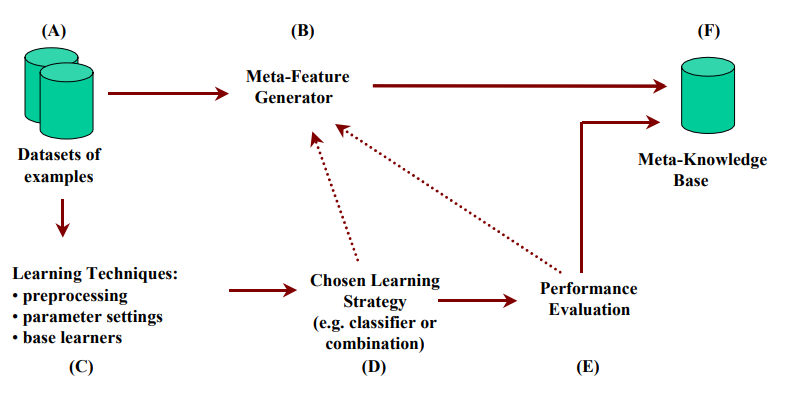
\includegraphics{Chapters/Images/MetaLearningAcquasition/MetaLearningAcquasition.PNG}}
\caption{An Example of Meta Learner Knowledge Acquisition}
\centering
Image borrowed from \cite{Vilalta} \\
Parameter setting not applicable in this experiment
\end{figure}

In advisory mode, the meta learning system makes use of the knowledge gathered in
the acquisition phase in order to suggest a best learning algorithm for a new
dataset. Meta features extracted from the dataset are ``matched'' with the
meta knowledge base to produce a recommendation regarding the best available
learning strategy \cite{Vilalta}.

What this entails is a mapping between meta features and an optimum base learning
strategy. In the case of this thesis, this mapping is accomplished via the $k$-means
algorithm, with the meta features being a set of standard statistical measures
in the case of the brute force and active strategies (these features are described
in section 3.3) and the meta features being ``learning curves'' in the case of the
curve comparison strategy (these curves are described in section 2.3.3).

\begin{figure}[h]
\resizebox{\columnwidth}{!}{%
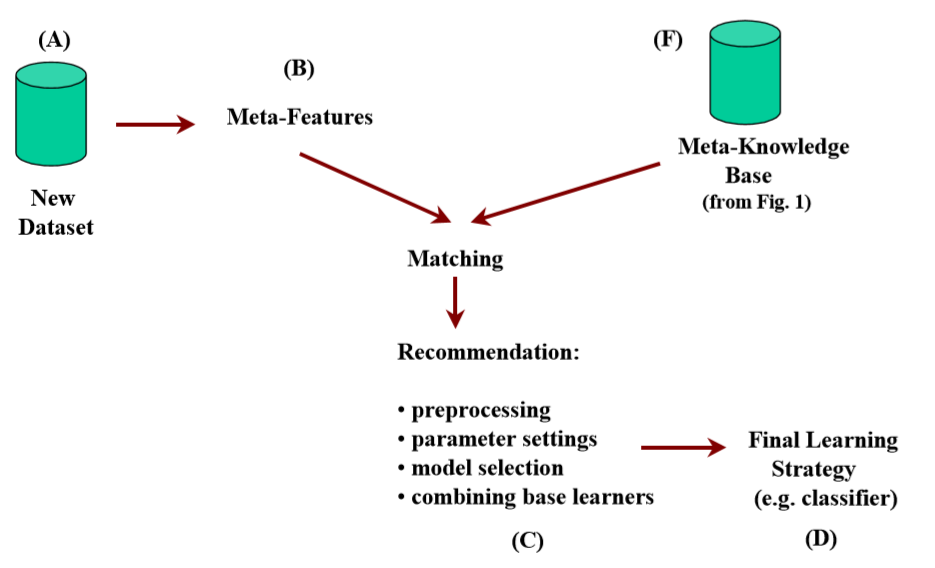
\includegraphics{Chapters/Images/MetaLearningAdvisory/MetaLearningAdvisory.PNG}
}
\caption{An Example of Meta Learner Advisory Mode}
\centering
Image borrowed from \cite{Vilalta} \\
Parameter setting not applicable in this experiment
\end{figure}

%-------------------------------------------------------------------------------------------
\section{Summary of the Compared Meta Learning Strategies}
In order to ascertain whether the NFL theorem applies to meta learning strategies,
we require a set of meta learning strategies with which to make run comparisons. The
meta learning strategies used in the experiment that comprises this thesis are described within
this section.
%-------------------------------------------------------------------------------------------
\subsection{Brute Force Metabase}
This is the most basic meta-machine learning algorithm. During the acquisition phase,  the
accuracies of the meta learner's producible machines for some metabase are gathered
and stored within a database. Classification of a new dataset $d_n$ during advisory
mode is accomplished via the usage of a clustering algorithm ($k$-Means in the case
of this experiment) and is used to find $d_m$, the dataset within the metabase
to which the new dataset $d_n$ is most similar. The algorithm which was found
to have had the greatest classification accuracy for the metabase dataset $d_m$
during acquisition will then be returned by the meta-learner.
\begin{figure}[h]
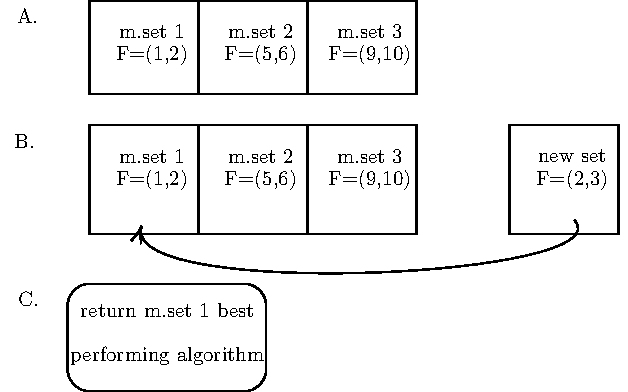
\includegraphics{Chapters/Images/BaseLearner/BaseLearner.pdf}
\caption{Example of base meta learning}
\centering
\begin{flushleft}
A. Metabase sets with given meta feature vectors \\
B. Classify new dataset by meta feature vector comparison \\
C. Return best algorithm of associated meta base set
\end{flushleft}
\end{figure}
%-------------------------------------------------------------------------------------------
\subsection{Active Meta Learning}
The second of the meta learning strategies implemented within this study, Active
Meta Learning is a meta learning technique  ``that reduces the cost of
generating Meta examples by selecting relevant Meta examples'' \cite{Bhatt}.
What this entails is a decision on what datasets to allow into a meta learner's
metabase during acquisition mode. Rather than analyze every candidate meta base
dataset, an active meta learner will analyze the next dataset with the highest
uncertainty. The relative uncertainty between two datasets is defined to be:
$$\delta(V_x,d_i,V_x,d_j) = \frac{|V_x,d_i - V_x,d_j|}{Max_{k\neq i}(V_x,d_k)- Min_{k\neq i}(V_x,d_k)},$$
where $V_x,d_k$ is the value of some meta parameter $V_x$ for dataset $d_k$,
$Max_{k\neq i}(V_x,d_k)$ is the maximum value of $V_x,d_k$ when dataset $i$ is
removed and $Min_{k\neq i}(V_x,d_k)$ is its corresponding minimum. Determining
which dataset has the overall highest uncertainty can be done via the following
procedure. First, sum the relative uncertainties for each dataset and
meta parameter combination. Then, rank the uncertainty scores of the datasets within
each meta parameter. After obtaining the uncertainty ranks within each parameter
for each dataset, sum the parameter ranks in order to obtain an overall
uncertainty rank for each dataset. Finally, select the parameter with the
highest rank for inclusion in the metabase. The equation representing the
overall uncertainty score in a specific meta parameter $V_x$ for dataset $d_i$ is
$$\delta(V_x,d_i) = \frac{\sum_{j\neq i} |V_x,d_i - V_x,d_j|}{Max_{k\neq i}(V_x,d_k)- Min_{k\neq i}(V_x,d_k)}.$$
\begin{figure}[h]
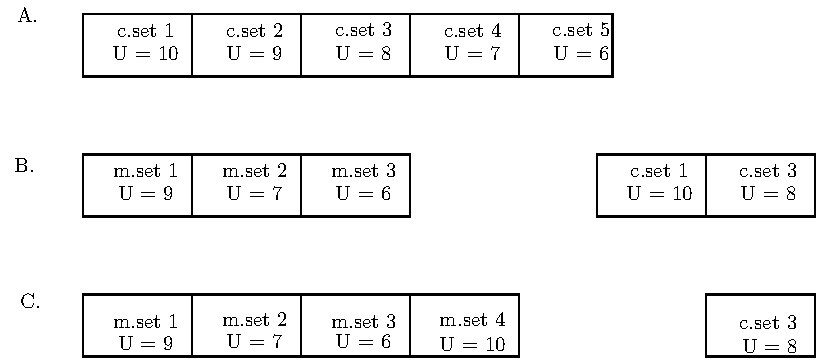
\includegraphics{Chapters/Images/ActiveLearner/ActiveLearner.pdf}
\caption{Example of active meta learning}
\centering
\begin{flushleft}
A. Set of candidate metabase sets \\
B. Random selection of half the original candidates \\
C. Inclusion of half remaining candidates by uncertainty comparison \\
\end{flushleft}
\end{figure}
%-----------------------------------------------------------------------------------------------
\subsection{Predicting Relative Performance of Classifiers from Samples}
Introduced in the paper ``Predicting Relative Performance of Classifiers from
Samples,'' the strategy of nearest learning curve comparison gathers run
statistics on the datasets within its metabase at various fractions of the full
size of the training portion of that dataset \cite{Leite}. It is then possible to plot a 2D
``learning curve,'' with the $x$ axis of such a graph being a specific fraction
of the training set and the $y$ axis of such a graph being the test classification
accuracy at that percent. The creation of these learning curves for each of the
datasets within the metabase is the work of this meta learning strategies
acquisition mode.

The categorization of new datasets during advisement mode can then be
accomplished in two steps. First, a model is trained on the new dataset with
some fractions of its training set using each candidate algorithm. These results
are then compared with the learning curves of each of the sets in the metabase.
The meta learner then returns the best algorithm of the dataset within the
metabase to which the new datasets learning curves is most similar. The
authors state that this process trains its meta learner in less time than a
brute force learner and that the resultant meta learner will also have a higher
classification accuracy than a brute force meta learner.

\begin{figure}[h]
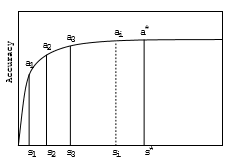
\includegraphics{Chapters/Images/LearningCurve/LearningCurve.PNG}
\caption{Example of a learning curve}
\centering
\begin{flushleft}
where: \\
A. Horizontal axis: Fractions of training set \\
B. Verticle axis: Test case accuracy for given set fraction \\
\end{flushleft}
Image borrowed from \cite{Leite}
\end{figure}
%----------------------------------------------------------------------------------------
\section{Summary of Producible Machines}
The strategies mentioned in the previous section all have advisory modes in which
a vector representation of an unprocessed dataset is consumed and a
prediction as to what algorithm would best be able to classify its data is made.
The machines that these strategies can choose from are the $k$-means clustering
algorithm, a neural network, a naive Bayes classifier, the support
vector machine, and regression. A brief description of each of these different
learning algorithms will comprise the rest of this chapter. For a more in-depth
discussion of the algorithms discussed within this chapter, the reader should consult
the appropriate chapter in Murphy's general purpose machine learning text
\cite{Murphy}.
%--------------------------------------------------------------------------------------------
\subsection{Linear Regression}
Linear regression is one of the most common and oldest machine learning
techniques. It asserts that the response is a linear function
of the inputs \cite{Murphy}. This relation takes the following form:
$$ y(\textbf{x}) = \textbf{w}^T\textbf{x} + \epsilon = \sum_{j=1}^{D}w_jx_j + \epsilon,$$
where $\textbf{w}^T\textbf{x}$ represents the inner or scalar product between the input vector $x$
and the model's weight vector $\textbf{w}^T$, and $\epsilon$ is the residual error
between our linear predictions and the true response.

To fit a linear regression model, the least squares approach is usually used.
Given some  ``overdetermined'' linear system (that is to say a system in which
there are more data points than parameters), one can write an expression for the
sum of squares of the system
$$S(\beta) = (y_1 - \beta x_1)^2 + (y_2 - \beta x_2)^2 + ... (y_n - \beta x_n)^n,$$
and then take the partial derivative of this sum of squares deviations with respect
to each of the components of $\beta$, set them to zero, then solve the resulting
equations to directly determine the values of the parameters that
minimize the sum of the squared errors of the system. With linear regression in
two dimensions (one dimension in the Independent variable and one dimension in
the Dependent variable, we see a system with two parameters:
$\beta_0 = y~intercept$ and $\beta_1 = slope$. If we had, for example, 3 data
points (2,1),(3,7), and (4,5) we would have the equations
$\beta_0 + 2*\beta_1 = 1$, $\beta_0 + 3*\beta_1 = 7$, and
$\beta_0 + 4*\beta_1 = 5$. The sum of squared errors would then be
 $S(\beta_0,\beta_1)= [1 - (\beta_0 + 2*\beta_1)]^2 + [7 - (\beta_0 + 3*\beta_1)]^2 + [5 - (\beta_0 + 4*\beta_1)]^2$
, which we could then differentiate with respect to $\beta_0$ and $\beta_1$, then
directly solve the resulting set of linear equations for the minimum of
the summed squares.
%--------------------------------------------------------------------------------------------
\subsection{Naive Bayes}
The Na\"{i}ve Bayes classifier algorithm uses Bayes rule to construct a classifier
that makes a simplifying assumption. Given a set of discrete-valued
features $x \in {1,...,K}^D$, we can calculate the class conditional density for
each feature, then, with our assumption of independence, generate a guess
at what the class should be for a new input, by multiplying the conditional
likelihood values for each of the new inputs features times the prior on the
desired to be known class, that is to say
$p(y|\textbf{x}) \propto p(y) \sum_{j}^{D}p(x_j|y)$.
The calculation of the posterior probability for a new example can be done
manually, or can be derived from distributions that are inferred from the
provided data. Consider, for example, a collection of data listing individuals
that did or did not purchase a house from a real estate agent, where, for some
reason or another, the only data remaining pertaining to these individuals are:
what their income level was, what their age was, and how far they have to or
would have had to drive to work from their new home.

Say, for example, we get a new datapoint: income: \$25,000, age: 30, distance: 10. In this
case the conditional likelihood of this data given a yes for each of the
individual features is 2/9, 1/9, and 2/9 respectively. The prior on yes is 1/3.
The marginal likelihoods of each of the individual features are 2/9, 1/9 and 2/9
respectively. As such, the posteriors for our new datapoint are
$p(y=yes|x)=\frac{(2/9)*(1/9)*(2/9)*(9/27)}{(6/27)*(3/27)*(6/27)} = \frac{0.00182}{0.00548} = 0.33$ and $p(y=no|x)=\frac{(4/18)(2/18)(4/18)(18/27)}{(6/27)(3/27)(6/27)} = \frac{0.0036}{0.00548} = 0.66$.

Note that $0.66 > 0.33$ and as such our classifier would label this datapoint
with a no, this individual is not likely to purchase a house.

%--------------------------------------------------------------------------------------------
\subsection{Support Vector Machine}
The support vector machine (SVM) is a binary classification algorithm that
attempts to find a hyperplane that separates the inputs within a given input
space with a maximum margin of separation between the hyperplane and the
``support vectors,'' those vectors on either side of the hyperplane
that are closest to it. To arrive at a form of the support vector machine that
can be used to classify new inputs, one first needs a representation of the
potential separating hyperplane $$y_i(\mathbf{w}*\mathbf{x}_i + b) > 1,$$ where
$y_i$ is the truth label of given training input $\bold{x}_i$, $\bold{w}$ is a vector
normal to our candidate separating hyperplane that represents how much
``weight'' is to be applied to an input, and $b$ is a bias constant representing
the threshold the weight/input product needs to pass before it is considered
classified. The distance of a given hyperplane can be determined by calculating
the difference between these previously mentioned ``support vectors'' in the
direction normal to this hyperplane. This difference can be calculated via the
following equation:
$$(\bold{x_{s+}}-\bold{x_{s-}})\bold{\frac{w}{||w||}},$$ where $\bold{x_{s+}}$
and $\bold{x_{s-}}$ are respectively positive and negative support vectors and
$\bold{\frac{w}{||w||}}$ is the unit vector in the direction normal to the hyper
plane towards the positive examples. The size of the margin is $2/||w||$. As
such, the discovery of a working SVM can be accomplished by solving a constrained
optimization problem in which the thing to be minimized is $1/2||w||^2$, subject
to the constraints $y_i(\bold{w}*\bold{x_i} + b) = 1$ for support vectors.
Crafting an expression of this constrained optimization that can be solved by a
computer can be done by taking the Lagrangian:
$$L(\bold{W},\bold{\lambda},\bold{Y}) = 1/2||\bold{w}||^2 \sum_{i=1}^{n}y_i(\bold{w}*\bold{x_i}+b)-1,$$
then taking care of the fact that the vector $w_o$ that determines the optimal
hyperplane can be written as a linear combination of the training vectors:
$w_{0}=\sum_{i=1}^{n}y_{i}\alpha_{i}^{0}\bold{x_i}$ \cite{Vapnik}. Swapping this
equation into the Lagrangian yields:
$$L = \sum \alpha_{i} - 1/2 \sum_{i}\sum_{j}\alpha_{i}\alpha_{j}y_{i}y_{j}(\bold{x_i}\cdot\bold{x_j}),$$
which can be optimized computationally.

This final form of the Lagrangian reveals the support vector machine's most
powerful attribute: the kernel. The optimization of the hyperplane within the
inputs depends only on the dot product of pairs of inputs; they do not appear
anywhere else in the Lagrangian other than the very end and then only so as
pairs of dot products. This fact allows the writing of a decision function on
new inputs: $$f(\bold{u}) = \sum_{i}^{N}\alpha_{i}y_{i}(\bold{x_i}\cdot\bold{u})+b,$$
where $\bold{u}$ is a vector whose label we do not know. The support vector
machine can use kernels to map input vectors into
non-linear high-dimensional feature space without actually calculating the
position of the vectors within that feature space \cite{Vapnik}. The kernel
accomplishes this by calculating the distance (or similarity)between two
input vectors in this space without reference to their exact position within
this higher space. This then allows the computation of a linear separation
between the points in this higher dimensional space which translates into a
non-linear separation for the vectors in their original lower dimensional space
where a separation might otherwise not have been discoverable.
%--------------------------------------------------------------------------------------------
\subsection{$k$-Means Clustering}
The objective of the $k$-means algorithm is to partition a dataset into k groups
such that the points within some group are all closer to
the mean of that group than they are to any other group. A clear
informal explanation of the work that the $k$-means algorithm performs
was given by James MacQueen in 1967: ``...the $k$-means procedure
consists of simply starting with k groups each of which consists of a
single random point, and thereafter adding each new point to the
group whose mean the new point is nearest. After a point is added to
a group, the mean of that group is adjusted in order to take account
of the new point. Thus at each stage the $k$-means are, in fact, the
means of the groups they represent'' \cite{MacQueen}. Formally stated,
given an integer $k$ and a set of $n$ data points in
$\mathbb{R}^{d}$ the $k$-means algorithm seeks to minimize $\Phi$, the
over all total summed in class distance between each point and its
closest center such that $\Phi = \sum_{x \in X} min_{c \in C}||{x-c^{2}}||$
\cite{Arthur}.

The $k$-means model is a type of Gaussian mixture model that is trained with a
procedure called expectation maximization. Given a set of distributions with
missing data, mixture models tend to have derivatives that are either difficult
to define or are entirely undefinable. On the other hand, the calculation of some
ML/MAP (maximum likelihood/maximum a posteriori) estimates for some set of models
can generally be done with little difficulty if every point within the
distributions is known (at which point our learner would have nothing to do) and
thus calculus would be unnecessary ($i.e.$, it would not matter that the derivative
cannot be defined). Expectation maximization uses this fact in order to obtain an
estimation of the ML/MAP indirectly. The algorithm consists of two steps. First,
an estimate as to what the expected value of the hidden data is based off the
current guess for the parameters is made. Then, the likelihood function for the
parameters is maximized under the assumption that the data discovered in the
previous step are complete, $i.e.$, that there are no longer any hidden data. These
steps are then repeated until some convergence criterion is met. The $k$-means is
exactly this type of algorithm, but with the covariance matrix
$\Sigma_{k} = \rho^{2}*I_{D}$ and the mixing weights $\Pi_{k} = 1/K$ all being fixed,
such that the only free parameters are the cluster centers $\mu_{k} \in \mathbb{R}^{D}$,
and such that the hidden data is the ground truth label of the data points.
%--------------------------------------------------------------------------------------------
\subsection{Neural Network}
A neural network is a type of machine learning algorithm that mimics
the inter-connectivity of animal brains in order to automatically
discover rules to classify given inputs. The neural network is one of the most
flexible learning algorithms within literature, so flexible in fact that it is
capable of approximating any continuous function \cite{Hornik}. As such, its
inclusion within a meta learning system is almost mandatory.  Generally,
a neural network system works by first being presented with a set of classified or
unclassified inputs. Said system will then attempt to
make a decision on these inputs on which an error value will then be
assigned. The system will then see some kind of correction function
applied to it. This process will continue until the system has
exhausted its supply of training data, at which point it will
hopefully have discovered a strong set of rules for performing whatever
work it is that it was designed to perform.

The type of neural network that will be used within this thesis is
what is called the feed-forward neural network (a.k.a. multilayer perceptron,
or MLP). The feed forward neural network is essentially a series of
logistic regression models stacked on top of each other, with the
final layer being either another logistic regression or linear
regression model depending on whether or not a classification or
regression problem is being solved \cite{Murphy}. The leftmost
layer of this stack is called the input layer and consists of a set of
neurons ${x_i|x_1,x_2,x_3,...,x_m}$ representing the input's
features. Each neuron in the hidden layer transforms the values from
the previous layer via weighted linear summation $w_1x_1 + w_2x_2 +...+w_mx_m$
which is then passed into a non-linear action function $g()$, such as the
logistic function or the hyperbolic tangent function. It is important to note
that $g$ must be non-linear, otherwise the entire model will collapse into a
large linear regression model of the form $y = w^T(Vx)$ \cite{Murphy}.

The multi-layer perceptrons created in this experiment will be trained
by an error propagation/training technique called backpropagation.
Backpropagation is a procedure that repeatedly adjusts the weights of the
connections in a neural network so as to minimize a measure of the difference
between the actual output vector of the net and the desired output
vector \cite{Rumelhart}. In order to accomplish this, the algorithm
adjusts the weights of the neural network by considering the error of
the outputs then minimizes this error via gradient descent with respect
to each of the weights within the network. Specifically, the gradient
vector of the negative log-likelihood error on the output neurons is
computed by use of the chain rule of calculus \cite{Murphy}. Say we
have a one layer neural network in which the hidden layer is described
by $\alpha^{L} = \sigma(w^{L}\alpha^{L-1} + b^{L}) = \sigma(z^{L})$,
where $L$ superscript refers to the hidden layer and $L-1$ refers
to the input layer of the network. The parameters of this network can
be said to be $\Theta = (V,W)$ where $V$ is the weight vector for the input
layer and $W$ is the weight vector for the hidden layer. The error (or
more specifically the costs function) of a such a network is given by:
$$J(\Theta ) = - \sum_n\sum_k(\hat{y}_{nk}(\Theta)-y_{nk})^2$$
in the case of regression, and via cross-entropy,
$$J(\Theta ) = - \sum_n\sum_ky_{nk}log\hat{y}_{nk}(\Theta),$$
in the case of classification. The gradient of this error $\nabla_{\Theta}J$
is found via the chain rule of calculus:
$$\frac{\partial C}{\partial
w^{L}} = \frac{\partial z^{L}}{\partial
w^{L}}\frac{\partial \alpha}{\partial z^{L}}\frac{\partial
  C}{\partial \alpha^{L}}.$$
This equation is easiest to understand if read from right to left.
Notice how in each stage the rates being compared are between nearest
elements, first the error to the output that produced it, then the output
to the element to which the non-linearity is applied, then finally the the
non-linearity receiving value to the weight vector. The result of this
calculation easily gives us the direction of the gradient, the negative of
which we will use to modify $w^{L}$ in a direction that will reduce the output
error. Reduction of the error of a multilayer perceptron with more
than one neuron in each layer works mostly the same way. Once again,
the chain rule of calculus is used in order to find the derivative of
the output error with respect to the weights of the connections
between the hidden layer before the output neurons and the output
neurons $\frac{\partial C}{\partial w^{L}_{n-j}}$, where $L$ is the
target neuron's layer (the last layer in this case), $n$ is the index of
a neuron within this layer, and $j$ is the index of the neuron in the
previous layer $L-1$ from which neuron $n$ is receiving input (note
that in this case the hyphen does not mean subtract, but rather
indicates that there is a connection between these neurons). For an output
neuron, its error is then given by:
$$\frac{\partial C}{\partial w^{L}_{n-j}} = \frac{\partial z^{L}_{j}}{\partial w^{L}_{n-j}}\frac{\partial \alpha^{L}_{j}}{\partial z^{L}_{j}}\frac{\partial C}{\partial \alpha^{L}_{j}},$$
with the error relative to neurons earlier in the network being calculable by
continuing usage of the chain rule.

%For an excellent and intuitive explanation of how neural networks work,
%pls consider viewing the animated overview of the method at 3Blue1Brown's
%youtube channel.
% WAY TOO INFORMAL!

%Chapter 3
\usepackage{amssymb}
\chapter{Overview of producable machines}
\label{Chapter3}
%----------------------------------------------------------------------------------------

% Define some commands to keep the formatting separated from the content
\newcommand{\keyword}[1]{\textbf{#1}}
\newcommand{\tabhead}[1]{\textbf{#1}}
\newcommand{\code}[1]{\texttt{#1}}
\newcommand{\file}[1]{\texttt{\bfseries#1}}
\newcommand{\option}[1]{\texttt{\itshape#1}}

%----------------------------------------------------------------------------------------
\section{Summary of producable machines}
The strategies mentioned in the previous section must be able to produce learning algorithms
to be considered metalearing machines. The machines that these strategies can produce are
the K-means clusterer, a neural network, a naive bayes classifier, the support vector machine,
and regression; with the results coming from the regression machine being cast into classificatory bins
from the real valued result that it would produce. An in depth description of each of these different
earning algorithms will comprise the rest of this chapter.
%--------------------------------------------------------------------------------------------
\section{Regression}
%--------------------------------------------------------------------------------------------
\section{K-Means clustering}
The objective of the k-means algorithm is to partition a dataset into
k groups such that the points within some group are all closest to
the mean of that group than they are to any other group. A clear
informal explanation of the work that the k-means algorith performs
was given by James McQueen in 1967: "...the k-means procedure
consists of simply starting with k groups each of which consists of a
single random point, and thereafter adding each new point to the
group whose mean the new point is nearest. After a point is added to
a group, the mean of that group is adjusted in order to take account
of the new point. Thus at each stage the k-means are, in fact, the
means of the groups the represent."\cite{McQueen} Formally stated, given an integer \textit{k} and a set of \textit{n} data points in $\mathbb{R}^{d}$
the K-means algorithm seeks to minimize  \Phi, the over all total summed in class distance between
each point and its closest center such that $$\mathbb\Phi = \sum_{x \in X} min_{c \in C}\left x-c \right^{2} $$
\cite{Arthur}
%--------------------------------------------------------------------------------------------
\section{Neural Networks}
A neural network is a type of machine learning algorithm that mimics
the interconnectivity of animal brains in order to automatically
discover rules to classify given inputs. Being that it is one of the most
flexible learning algorithms within literature (actually able to
approximate any continuous function)\cite{Hornik}, its inclusion within a
metalearning system is almost mandatory.  Genrally, such a system
works by first being presented with a set of classified or
unclassified inputs. Said neural network system will then attempt to
make a decision on these inputs on which an error value will then be
assigned. The system will then see some kind of correction function
applied to it. This process will continue until the system has
exhausted its supply of training data, at which point it will
hopefully have discovered a strong set of rules for peforming whatever
work it is that it was designed to perform.

The type of neural network that will be used within this thesis is
what is called the feed-forward neural network (multilayer perceptron
aka MLP). The feed forward neural network is essentially a series of
logistic regression models stacked on top of each other, with the
final layer being either another logicstic regression or linear
regression model depending on whether or not a classification or
regression problem is being solved.\cite{Murphy}. The leftmost
layer of this stack is called the input layer and consists of a set of
neurons {x_i|x_1,x_2,x_3...,x_m} representing the input's
features. Each neuron in the hidden layer transforms the values from
the previous layer via weighted linear summation w_1X_1 + w_2x_2 +
...w_mx_m \cite{Scikit} which is then passed into a non linear-action
function g(), such as the logistic function or the hyperbolic tangent
function. It is important to note that g must be non-linear, otherwise
the entire model will collapse into a large linear regression model of
the form y = w^T(Vx). \cite{Murphy}

In order to train the MLP it provides, sci-kit learn uses an error
propagation/training technique called backpropagation. Backpropagation
is a procedure that repeatedly adjusts the weights of the connections
in a neural network so as to minimize a measure of the difference
between the actual output vector of the net and the desired output
vector. \cite{Rumelhart}. In order to accomplish this, the algorithm
adjusts the weights of the nerual network by considering the error of
the outputs then minimizes this error via gradient decent with respect
to each of the weights within the network. Specifically, the gradient
vector of the negative log likelihood error on the output neurons is
computed by use of the chain rule of calculus.\cite{Murphy}.Say we
have a one layer neural network in which the hidden layer is described
by $$\alpha^{L} = \sigma(w^{L}\alpha^{L-1} + b^{L}) = \sigma(z^{L})$$
where $$L$$ superscript refers to the hidden layer and $$L-1$$ refers
to the input layer of the network. The parameters of this network can
be said to be $$\Theta = (V,W)$$ where V = weight vector for the input
layer and W is the weight vector for the hidden layer. The error (or
more specifically the costs function) of a such a network is given by $$J(\Theta ) =
- \sum_n\sum_k(\hat{y}_{nk}(\Theta)-y_{nk})^2$$ in the case of
regression and via cross entropy $$J(\Theta ) =
- \sum_n\sum_ky_{nk}log\hat{y}_{nk}(\Theta)$$ in the case of
classification. The gradient of this error $$\nabla_{\Theta}J$$ is
found via the chain rule of calculus: $$\frac{\partial C}{\partial
w^{L}} = \frac{\partial z^{L}}{\partial
w^{L}}\frac{\partial \alpha}{\partial z^{L}}\frac{\partial
C}{\partial \alpha^{L}}$$. This equation is easiest to understand if
read from right to left, notice how in each stage the rates being
compared are between nearest elements, first the error to the output
that produced it, then the output to the element to which the
non-linearity is applied, then finally the the non-linerity recieving
value to the weight vector. The result of this calculation easily
gives us the direction of the gradient, the negative of which we will
use to modify $$w^{L}$ in a direction that will reduce the output
error. Reduction of the error of a multilayer perceptron with more
than one neuron in each layer works mostly the same way. Once again,
the chain rule of calculus is used in order to find the derivative of
the output error with respect to the weights of the connections
between the hidden layer before the output neurons and the output
neurons $$\frac{\partial C}{\partial w^{L}_{n-j}}$$ where $$L$$ is the
target neurons layer (the last layer in this case), n is the index of
a neuron within this layer, and j is the index of the neuron in the
previous layer $$L-1$$ from which neuron n is recieving input (note
that in this case the hyphen does not mean subtract but rather
indicates that their is a connection between these
neurons). For an output neuron, its error is then given by $$\frac{\partial C}{\partial
w^{L}_{n-j}} = \frac{\partial z^{L}_{j}}{\partial
w^{L}_{n-j}}\frac{\partial \alpha^{L}_{j}}{\partial z^{L}_{j}}\frac{\partial
C}{\partial \alpha^{L}_{j}}$$, with the error relative to neurons
earlier in the network being calculable by continuing usage of the
chain rule. \begin{figure}\end{figure}. For an excellent and intuitive
explanation of how neural networks work, pls consider viewing the
animated overview of the method at 3Blue1Brown's youtube channel.
%--------------------------------------------------------------------------------------------
\section{Naive Bayes}

%%Chapter 4
\chapter{Research Findings}
\label{Chapter4}
\section{Run Results and Analysis Tools}
If the no free lunch theorem applies to  meta-learning strategies, we
should see near equal performance across a variety of meta-set collections.
We will call this assertion the null hypothesis, that is to say our null
hypothesis is that the meta-learning strategies used in this experiment
are equal.

In order to test the null hypothesis, 30 such samples of the kind described
in Chapter 3 were collected. The metrics of interest on these samples are
contained in the tables within this chapter. How often the algorithms placed
first, second, or third can be seen in table 4.1. The average of these
placements across all samples, i.e the algorithms average placements, can be
seen in table 4.2. Table 4.3 contains the proportion of probability for the
results contained in table 4.1. Table 4.4 contains the average of the
proportion of probabilities contained in table 4.3 across all samples.
Table 4.5 contains the standard deviations of the placement values for the
meta-algorithms. Table 4.6 contains the t scores of each of the values present
in table 4.1. Table 4.7 contains the average of the t scores contained in
table 4.6 across all samples and it is this table that I use later to draw the
conclusion that the null hypothesis may be safely rejected.

\begin{table}
\begin{tabular}{lrrrrrrrrr}
\toprule

     & \multicolumn{3}{c} {GuessesActive}  & \multicolumn{3}{c}{GuessesEx}  & \multicolumn{3}{c}{GuessesSamp}  \\
     &   First &  Second &  Third &         First &  Second  &  Third &           First &  Second &  Third \\
\midrule
sample 1   &             1 &  4 &  5 &         6 &  2 &  2 &           3 &  4 &  3 \\
sample 2   &             1 &  4 &  5 &         5 &  2 &  3 &           4 &  4 &  2 \\
sample 3   &             1 &  3 &  6 &         7 &  3 &  0 &           2 &  4 &  4 \\
sample 4   &             1 &  5 &  4 &         6 &  3 &  1 &           3 &  2 &  5 \\
sample 5   &             0 &  6 &  4 &         8 &  2 &  0 &           2 &  2 &  6 \\
sample 6   &             3 &  3 &  4 &         5 &  4 &  1 &           2 &  3 &  5 \\
sample 7   &             4 &  3 &  3 &         4 &  4 &  2 &           2 &  3 &  5 \\
sample 8   &             2 &  3 &  5 &         7 &  2 &  1 &           1 &  5 &  4 \\
sample 9   &             1 &  3 &  6 &         3 &  5 &  2 &           6 &  2 &  2 \\
sample 10  &             0 &  4 &  6 &         7 &  3 &  0 &           3 &  3 &  4 \\
sample 11  &             0 &  6 &  4 &         7 &  3 &  0 &           3 &  1 &  6 \\
sample 12 &             1 &  5 &  4 &         7 &  2 &  1 &           2 &  3 &  5 \\
sample 13 &             3 &  3 &  4 &         5 &  4 &  1 &           2 &  3 &  5 \\
sample 14 &             2 &  5 &  3 &         6 &  3 &  1 &           2 &  2 &  6 \\
sample 15 &             2 &  1 &  7 &         4 &  6 &  0 &           4 &  3 &  3 \\
sample 16 &             1 &  5 &  4 &         6 &  0 &  4 &           3 &  5 &  2 \\
sample 17 &             1 &  4 &  5 &         6 &  4 &  0 &           3 &  2 &  5 \\
sample 18 &             1 &  3 &  6 &         8 &  1 &  1 &           1 &  6 &  3 \\
sample 19 &             1 &  4 &  5 &         7 &  3 &  0 &           2 &  3 &  5 \\
sample 20 &             2 &  4 &  4 &         6 &  2 &  2 &           2 &  4 &  4 \\
sample 21 &             1 &  2 &  7 &         4 &  6 &  0 &           5 &  2 &  3 \\
sample 22 &             3 &  3 &  4 &         2 &  7 &  1 &           5 &  0 &  5 \\
sample 23 &             3 &  4 &  3 &         6 &  4 &  0 &           1 &  2 &  7 \\
sample 24 &             3 &  3 &  4 &         4 &  4 &  2 &           3 &  3 &  4 \\
sample 25 &             2 &  6 &  2 &         7 &  3 &  0 &           1 &  1 &  8 \\
sample 26 &             1 &  3 &  6 &         6 &  2 &  2 &           3 &  5 &  2 \\
sample 27 &             7 &  2 &  1 &         3 &  5 &  2 &           0 &  3 &  7 \\
sample 28 &             0 &  5 &  5 &         7 &  2 &  1 &           3 &  3 &  4 \\
sample 29 &             1 &  2 &  7 &         4 &  5 &  1 &           5 &  3 &  2 \\
sample 30 &             2 &  6 &  2 &         4 &  3 &  3 &           4 &  1 &  5 \\
\bottomrule
\end{tabular}
\caption{Placement results}
\caption*{How well the meta-algorithms faired with given sample}
\end{table}


\begin{table}
\begin{tabular}{lrrr}
\toprule
{} &  GuessesActive &  GuessesEx &  GuessesSamp \\
\midrule
First  &           1.70 &        3.8 &         4.50 \\
Second &           5.57 &        3.3 &         1.13 \\
Third  &           2.73 &        2.9 &         4.37 \\
\bottomrule
\end{tabular}
\caption{Average placement results across all samples}
\end{table}

Each of the meta-set collections contains 10 basesets and the experiment
compares the performance of 3 meta-learning algorithms. As such, the expected
average number of first, second, and third place finishes given that the
meta-learning algorithms are equal is 3.3. The values seen within the placement
counts table given equal meta-learning algorithms should more often than not be
either 3 or 4 and the averages of the placements across all samples should all
be near 3.3. Instead, it appears that the sampler performed the best,
with an average number of first place finshes of 4.5. Moreover most of the
averages present in table 4.2 seem to be farther away from the expected value of
3.3 than one would intuitively expect if the meta-learning algorithms were
truly equal. Whether or not these results fall far enough outside
expectation in order to reject the null hypothesis requires analysis with the
machinary of classical statistics. Two well established hypothesis testing
measures are the method of calculating sampling distribution probabilities and
t score analysis. A brief description of each of these statistical methods
follows.

\subsection{Exact Sampling Distribution}
The following description losely follows the procedure described in \cite{Cohen}.
In it, the author asks the reader to imagine testing a coin to see whether or
not it is fair, flipping the coin 1,2,..N times. He then asks the reader to
consider whether some proportion of heads is actually fair from 0/N, 1/N.., N/N
heads. The propability that some proportion of heads p = i/N is fair can be
calculated exactly with the binomial distribution
$$\frac{N!}{i!(N-i)!}r^{i}(1-r)^{N-i}$$
This situation is analogous to the number of first, second, or third place
finishes some meta-algorithm obtained in this thesis experiment. The probabilty
of proportions for each of the meta-learning algorithms can be seen in table 4.3
and the average of these proportions across all samples can be seen in table 4.4.

\begin{table}
\begin{tabular}{lrrrrrrrrr}
\toprule
 & \multicolumn{3}{l}{GuessesActive} & \multicolumn{3}{l}{GuessesEx} & \multicolumn{3}{l}{GuessesSamp} \\
 &             First &     Second &     Third &   First &     Second &     Third &     First &     Second &  Third \\
\midrule
sample 1  &          0.09 &  0.23 &  0.14 &      0.06 &  0.20 &  0.20 &        0.26 &  0.23 &  0.26 \\
sample 2  &          0.09 &  0.23 &  0.14 &      0.14 &  0.20 &  0.26 &        0.23 &  0.23 &  0.20 \\
sample 3  &          0.09 &  0.26 &  0.06 &      0.02 &  0.26 &  0.02 &        0.20 &  0.23 &  0.23 \\
sample 4  &          0.09 &  0.14 &  0.23 &      0.06 &  0.26 &  0.09 &        0.26 &  0.20 &  0.14 \\
sample 5  &          0.02 &  0.06 &  0.23 &      0.00 &  0.20 &  0.02 &        0.20 &  0.20 &  0.06 \\
sample 6  &          0.26 &  0.26 &  0.23 &      0.14 &  0.23 &  0.09 &        0.20 &  0.26 &  0.14 \\
sample 7  &          0.23 &  0.26 &  0.26 &      0.23 &  0.23 &  0.20 &        0.20 &  0.26 &  0.14 \\
sample 8  &          0.20 &  0.26 &  0.14 &      0.02 &  0.20 &  0.09 &        0.09 &  0.14 &  0.23 \\
sample 9  &          0.09 &  0.26 &  0.06 &      0.26 &  0.14 &  0.20 &        0.06 &  0.20 &  0.20 \\
sample 10 &          0.02 &  0.23 &  0.06 &      0.02 &  0.26 &  0.02 &        0.26 &  0.26 &  0.23 \\
sample 11 &          0.02 &  0.06 &  0.23 &      0.02 &  0.26 &  0.02 &        0.26 &  0.09 &  0.06 \\
sample 12 &          0.09 &  0.14 &  0.23 &      0.02 &  0.20 &  0.09 &        0.20 &  0.26 &  0.14 \\
sample 13 &          0.26 &  0.26 &  0.23 &      0.14 &  0.23 &  0.09 &        0.20 &  0.26 &  0.14 \\
sample 14 &          0.20 &  0.14 &  0.26 &      0.06 &  0.26 &  0.09 &        0.20 &  0.20 &  0.06 \\
sample 15 &          0.20 &  0.09 &  0.02 &      0.23 &  0.06 &  0.02 &        0.23 &  0.26 &  0.26 \\
sample 16 &          0.09 &  0.14 &  0.23 &      0.06 &  0.02 &  0.23 &        0.26 &  0.14 &  0.20 \\
sample 17 &          0.09 &  0.23 &  0.14 &      0.06 &  0.23 &  0.02 &        0.26 &  0.20 &  0.14 \\
sample 18 &          0.09 &  0.26 &  0.06 &      0.00 &  0.09 &  0.09 &        0.09 &  0.06 &  0.26 \\
sample 19 &          0.09 &  0.23 &  0.14 &      0.02 &  0.26 &  0.02 &        0.20 &  0.26 &  0.14 \\
sample 20 &          0.20 &  0.23 &  0.23 &      0.06 &  0.20 &  0.20 &        0.20 &  0.23 &  0.23 \\
sample 21 &          0.09 &  0.20 &  0.02 &      0.23 &  0.06 &  0.02 &        0.14 &  0.20 &  0.26 \\
sample 22 &          0.26 &  0.26 &  0.23 &      0.20 &  0.02 &  0.09 &        0.14 &  0.02 &  0.14 \\
sample 23 &          0.26 &  0.23 &  0.26 &      0.06 &  0.23 &  0.02 &        0.09 &  0.20 &  0.02 \\
sample 24 &          0.26 &  0.26 &  0.23 &      0.23 &  0.23 &  0.20 &        0.26 &  0.26 &  0.23 \\
sample 25 &          0.20 &  0.06 &  0.20 &      0.02 &  0.26 &  0.02 &        0.09 &  0.09 &  0.00 \\
sample 26 &          0.09 &  0.26 &  0.06 &      0.06 &  0.20 &  0.20 &        0.26 &  0.14 &  0.20 \\
sample 27 &          0.02 &  0.20 &  0.09 &      0.26 &  0.14 &  0.20 &        0.02 &  0.26 &  0.02 \\
sample 28 &          0.02 &  0.14 &  0.14 &      0.02 &  0.20 &  0.09 &        0.26 &  0.26 &  0.23 \\
sample 29 &          0.09 &  0.20 &  0.02 &      0.23 &  0.14 &  0.09 &        0.14 &  0.26 &  0.20 \\
sample 30 &          0.20 &  0.06 &  0.20 &      0.23 &  0.26 &  0.26 &        0.23 &  0.09 &  0.14 \\
\bottomrule
\end{tabular}
\caption{Placement results proportion probabilities}
\caption*{Proportion probabilities of placement results if the null hypothesis were true}
\end{table}


\begin{table}
\begin{tabular}{lrrr}
\toprule
{} &  GuessesActive &  GuessesEx &  GuessesSamp \\
\midrule
First  &        0.13 &       0.19 &         0.16 \\
Second &        0.10 &       0.19 &         0.11 \\
Third  &        0.19 &       0.20 &         0.16 \\
\bottomrule
\end{tabular}
\caption{Average of proportion probabilities across all samples}
\end{table}

We can calculate the probability of drawing either of the values closest
to expectation, 3 or 4, by use of the previously mentioned binomial distribution,
with $N = 10$, $r = 0.33$, and $i$ being either 3 or 4. The values we get for
the propabilities of the most expected values are then 0.26 and 0.22
respectively. The average of all values within this table is
0.15, significantly lower than the probability of the expected value.
Still, this is not enough to reject the null hypothesis as proportion
probability analysis does not come with a rejection criteria.

\subsection{t score}
$t$ score analysis is a form of hypothesis testing that allows one to determine
whether or not some result emerged from some given distribution via consideration
of how many standard deviations the result deviates from the mean of said given
distribution. Its equation has the form:
$$t =\frac{\overline{x}-\mu}{\hat{\sigma}_{\overline{x}}} = \frac{\overline{x}-\mu}{\frac{s}{\sqrt{N}}}$$
where $s$ is the sample standard deviation, $N$ is the number of samples,
$\overline{x}$ is an individual samples mean/calculated value, and $\mu$ is
the mean of the distribution of comparison.

The decision as to whether or not a specific $t$ score value implies a result
is from a different distribution depends on how many samples were used in the
calculation of the sample mean and on what the desired confidence interval is.
The critical threshold used in order to make this decision is gained by the use
of $t$ distribution table. In the case where 30 samples are used and the desired
margin of error is 5\%, the critical thresholds for a two tailed $t$ test are
-2.042 and 2.042. If the averaged values of the $t$ scores falls outside of
these bounds then we can reject the null hypothesis with a 5 \% margin of error.
The standard deviations and $t$ scores for each of the samples can be seen in
table 4.4. Taking the average of the absolute value of each of these $t$ scores
yeilds 5.11. We can thus comfortably reject the null hypothesis.


\begin{table}
\begin{tabular}{lrrr}
\toprule
{} &  GuessesActive &  GuessesEx &  GuessesSamp \\
\midrule
First  &           1.42 &       1.30 &     1.48 \\
Second &           1.54 &       1.53 &     1.06 \\
Third  &           1.36 &       1.33 &     1.58 \\
\bottomrule
\end{tabular}
\caption{Placement results standard deviations across all samples}
\end{table}


\begin{table}
\begin{tabular}{lrrrrrrrrr}
\toprule
algorithms & \multicolumn{3}{l}{GuessesActive} & \multicolumn{3}{l}{GuessesEx} & \multicolumn{3}{l}{GuessesSamp} \\
positions &  First &   Second &    Third &    First &  Second &  Third &    First &  Second &  Third \\
\midrule
sample 1  &        -10.41 &   3.24 &   7.13 &     10.93 &  -5.51 &  -7.98 &       -1.54 &   3.18 &  -1.33 \\
sample 2  &        -10.41 &   3.24 &   7.13 &      6.83 &  -5.51 &  -2.00 &        3.09 &   3.18 &  -5.33 \\
sample 3  &        -10.41 &  -1.62 &  11.41 &     15.04 &  -1.38 & -19.96 &       -6.18 &   3.18 &   2.67 \\
sample 4  &        -10.41 &   8.10 &   2.85 &     10.93 &  -1.38 & -13.97 &       -1.54 &  -6.36 &   6.67 \\
sample 5  &        -14.87 &  12.96 &   2.85 &     19.14 &  -5.51 & -19.96 &       -6.18 &  -6.36 &  10.67 \\
sample 6  &         -1.49 &  -1.62 &   2.85 &      6.83 &   2.75 & -13.97 &       -6.18 &  -1.59 &   6.67 \\
sample 7  &          2.97 &  -1.62 &  -1.43 &      2.73 &   2.75 &  -7.98 &       -6.18 &  -1.59 &   6.67 \\
sample 8  &         -5.95 &  -1.62 &   7.13 &     15.04 &  -5.51 & -13.97 &      -10.81 &   7.95 &   2.67 \\
sample 9  &        -10.41 &  -1.62 &  11.41 &     -1.37 &   6.89 &  -7.98 &       12.36 &  -6.36 &  -5.33 \\
sample 10 &        -14.87 &   3.24 &  11.41 &     15.04 &  -1.38 & -19.96 &       -1.54 &  -1.59 &   2.67 \\
sample 11 &        -14.87 &  12.96 &   2.85 &     15.04 &  -1.38 & -19.96 &       -1.54 & -11.13 &  10.67 \\
sample 12 &        -10.41 &   8.10 &   2.85 &     15.04 &  -5.51 & -13.97 &       -6.18 &  -1.59 &   6.67 \\
sample 13 &         -1.49 &  -1.62 &   2.85 &      6.83 &   2.75 & -13.97 &       -6.18 &  -1.59 &   6.67 \\
sample 14 &         -5.95 &   8.10 &  -1.43 &     10.93 &  -1.38 & -13.97 &       -6.18 &  -6.36 &  10.67 \\
sample 15 &         -5.95 & -11.34 &  15.69 &      2.73 &  11.02 & -19.96 &        3.09 &  -1.59 &  -1.33 \\
sample 16 &        -10.41 &   8.10 &   2.85 &     10.93 & -13.77 &   3.99 &       -1.54 &   7.95 &  -5.33 \\
sample 17 &        -10.41 &   3.24 &   7.13 &     10.93 &   2.75 & -19.96 &       -1.54 &  -6.36 &   6.67 \\
sample 18 &        -10.41 &  -1.62 &  11.41 &     19.14 &  -9.64 & -13.97 &      -10.81 &  12.72 &  -1.33 \\
sample 19 &        -10.41 &   3.24 &   7.13 &     15.04 &  -1.38 & -19.96 &       -6.18 &  -1.59 &   6.67 \\
sample 20 &         -5.95 &   3.24 &   2.85 &     10.93 &  -5.51 &  -7.98 &       -6.18 &   3.18 &   2.67 \\
sample 21 &        -10.41 &  -6.48 &  15.69 &      2.73 &  11.02 & -19.96 &        7.72 &  -6.36 &  -1.33 \\
sample 22 &         -1.49 &  -1.62 &   2.85 &     -5.47 &  15.15 & -13.97 &        7.72 & -15.91 &   6.67 \\
sample 23 &         -1.49 &   3.24 &  -1.43 &     10.93 &   2.75 & -19.96 &      -10.81 &  -6.36 &  14.67 \\
sample 24 &         -1.49 &  -1.62 &   2.85 &      2.73 &   2.75 &  -7.98 &       -1.54 &  -1.59 &   2.67 \\
sample 25 &         -5.95 &  12.96 &  -5.71 &     15.04 &  -1.38 & -19.96 &      -10.81 & -11.13 &  18.67 \\
sample 26 &        -10.41 &  -1.62 &  11.41 &     10.93 &  -5.51 &  -7.98 &       -1.54 &   7.95 &  -5.33 \\
sample 27 &         16.36 &  -6.48 &  -9.99 &     -1.37 &   6.89 &  -7.98 &      -15.45 &  -1.59 &  14.67 \\
sample 28 &        -14.87 &   8.10 &   7.13 &     15.04 &  -5.51 & -13.97 &       -1.54 &  -1.59 &   2.67 \\
sample 29 &        -10.41 &  -6.48 &  15.69 &      2.73 &   6.89 & -13.97 &        7.72 &  -1.59 &  -5.33 \\
sample 30 &         -5.95 &  12.96 &  -5.71 &      2.73 &  -1.38 &  -2.00 &        3.09 & -11.13 &   6.67 \\
\bottomrule
\end{tabular}
\caption{Placement results t scores}
\caption*{t score for each individual placement result}
\end{table}


\begin{table}
\begin{tabular}{lrrr}
\toprule
{} &  GuessesActive &  GuessesEx &  GuessesSamp \\
\midrule
First  &      -7.29 &       2.27 &         4.99 \\
Second &       9.16 &      -0.14 &       -13.17 \\
Third  &      -2.78 &      -2.07 &         4.13 \\
\bottomrule
\end{tabular}
\caption{Average of t scores across all samples}
\end{table}

%%Chapter 5
\chapter{Conclusion and Future Work}
\label{Chapter5}
In this thesis, I proposed that the no free lunch hypothesis might not apply to
meta learning algorithms. In order to test this hypothesis, I first built a
system to determine the accuracy of three meta learning strategies:
Exhaustive, Active, and Sampling. To use these strategies, a base of
datasets would first be randomly chosen from the collection of all available
datasets that had been gathered from the UCI Irvine data repository.
Each strategy would then be carried out on the metabase and make an
estimate as to what algorithm would result in the highest classification
accuracy. Each algorithm would make this guess for each dataset in the
collection of available datasets excluding the datasets within the current
metabase. A new metabase would then be chosen at random and the process would be
repeated 9 more times, giving a number between 0 and 10 for how many times
each algorithm got the first, second, or third most correct guesses.
This process was repeated 30 times, resulting in 30 samples. $t$ test analysis
was then performed, giving an average among the absolute values of each of
the position $t$ scores of 5.11, allowing us to reject the null
hypothesis at a 5 percent $p$ value.

Future work could involve repeat runs of the system described in this thesis
with more datasets, which would test the results in a wider variety of problem
domains, therefore strengthening the results. Other interesting variations of
this experiment could come from testing the results with different meta features,
testing the results with noisy datasets, and even testing the results with
artificially generated datasets. One could also test the results of this
procedure with an intermediary parameter tuning step, that is to say
we could tune the parameters of the various base algorithms to fit the domain
of the dataset currently being analyzed. Also, a future researcher might
choose to vary the algorithm used to classify the meta features, as here we
only make use of the $k$-means clustering algorithm to make our choice from the meta
features of our modified meta bases. The selection of a different algorithm
could change the results.


\printbibliography
%----------------------------------------------------------------------------------------
%	THESIS CONTENT - APPENDICES
%----------------------------------------------------------------------------------------

\appendix % Cue to tell LaTeX that the following "chapters" are Appendices

% Include the appendices of the thesis as separate files from the Appendices folder
% Uncomment the lines as you write the Appendices

% Appendix A

\chapter{Frequently Asked Questions} % Main appendix title

\label{AppendixA} % For referencing this appendix elsewhere, use \ref{AppendixA}

\section{How do I change the colors of links?}

The color of links can be changed to your liking using:

{\small\verb!\hypersetup{urlcolor=red}!}, or

{\small\verb!\hypersetup{citecolor=green}!}, or

{\small\verb!\hypersetup{allcolor=blue}!}.

\noindent If you want to completely hide the links, you can use:

{\small\verb!\hypersetup{allcolors=.}!}, or even better: 

{\small\verb!\hypersetup{hidelinks}!}.

\noindent If you want to have obvious links in the PDF but not the printed text, use:

{\small\verb!\hypersetup{colorlinks=false}!}.

%\include{Appendices/AppendixB}
%\include{Appendices/AppendixC}

%----------------------------------------------------------------------------------------

\end{document}
